\documentclass[12pt]{article}

\usepackage{graphicx} % Allows including images
\usepackage{booktabs} % Allows the use of \toprule, \midrule and \bottomrule in tables
\usepackage{amsmath}
\usepackage{amsfonts}
\usepackage{ifthen}
\usepackage{amssymb}
\usepackage{amsbsy}
\usepackage{bm}
\usepackage{ulem}
\usepackage{float}
\usepackage{latexsym}
\usepackage{comment}
\usepackage{graphicx}
\usepackage{amstext}
\usepackage{latexsym}
\usepackage{arydshln}
\usepackage{longtable}
\usepackage{enumerate}
\usepackage{multirow}
\usepackage{cases}
\usepackage{geometry}
\usepackage{mathtools}
\usepackage{subeqnarray}
\usepackage{textcomp}
\usepackage{hyperref}
%\usepackage{subfigure}
\usepackage{url}
\usepackage{threeparttable}
\usepackage{xr}
\usepackage{multirow}
\usepackage{wrapfig}
\usepackage{lscape}
\usepackage{rotating}
\usepackage{subcaption}
\usepackage{epstopdf}
\usepackage{verbatim}
\usepackage{xcolor}
\usepackage[sort&compress]{natbib}
\usepackage{bm}


\captionsetup{font={small}}
\geometry{left=2.0cm, right=2.0cm, top=2.5cm, bottom=2.5cm}

\title{EE526 Homework 5}

\author{Xingche Guo}

\date{\today}

\linespread{1.3}
\begin{document}
\maketitle

%%%%%%%%%%%%%%%%%%%%%%
\section*{Problem 1}

\begin{figure}[h] 
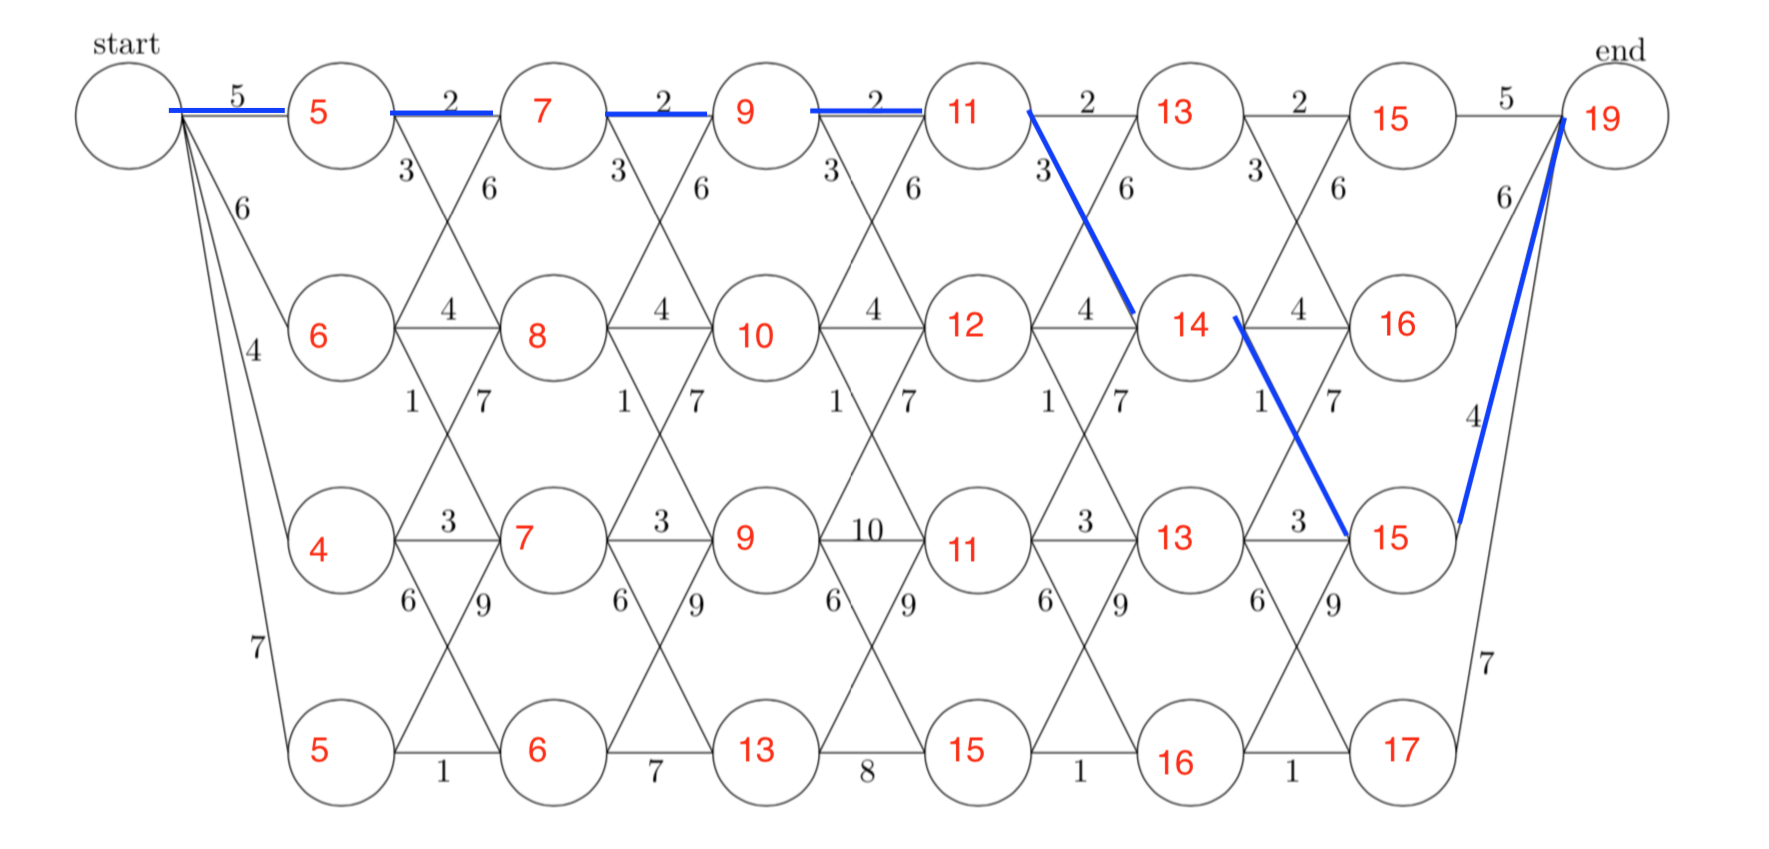
\includegraphics[width=1.0\textwidth]{prob1_1}
\caption{Shortest Path}
\end{figure}


\begin{figure}[h] 
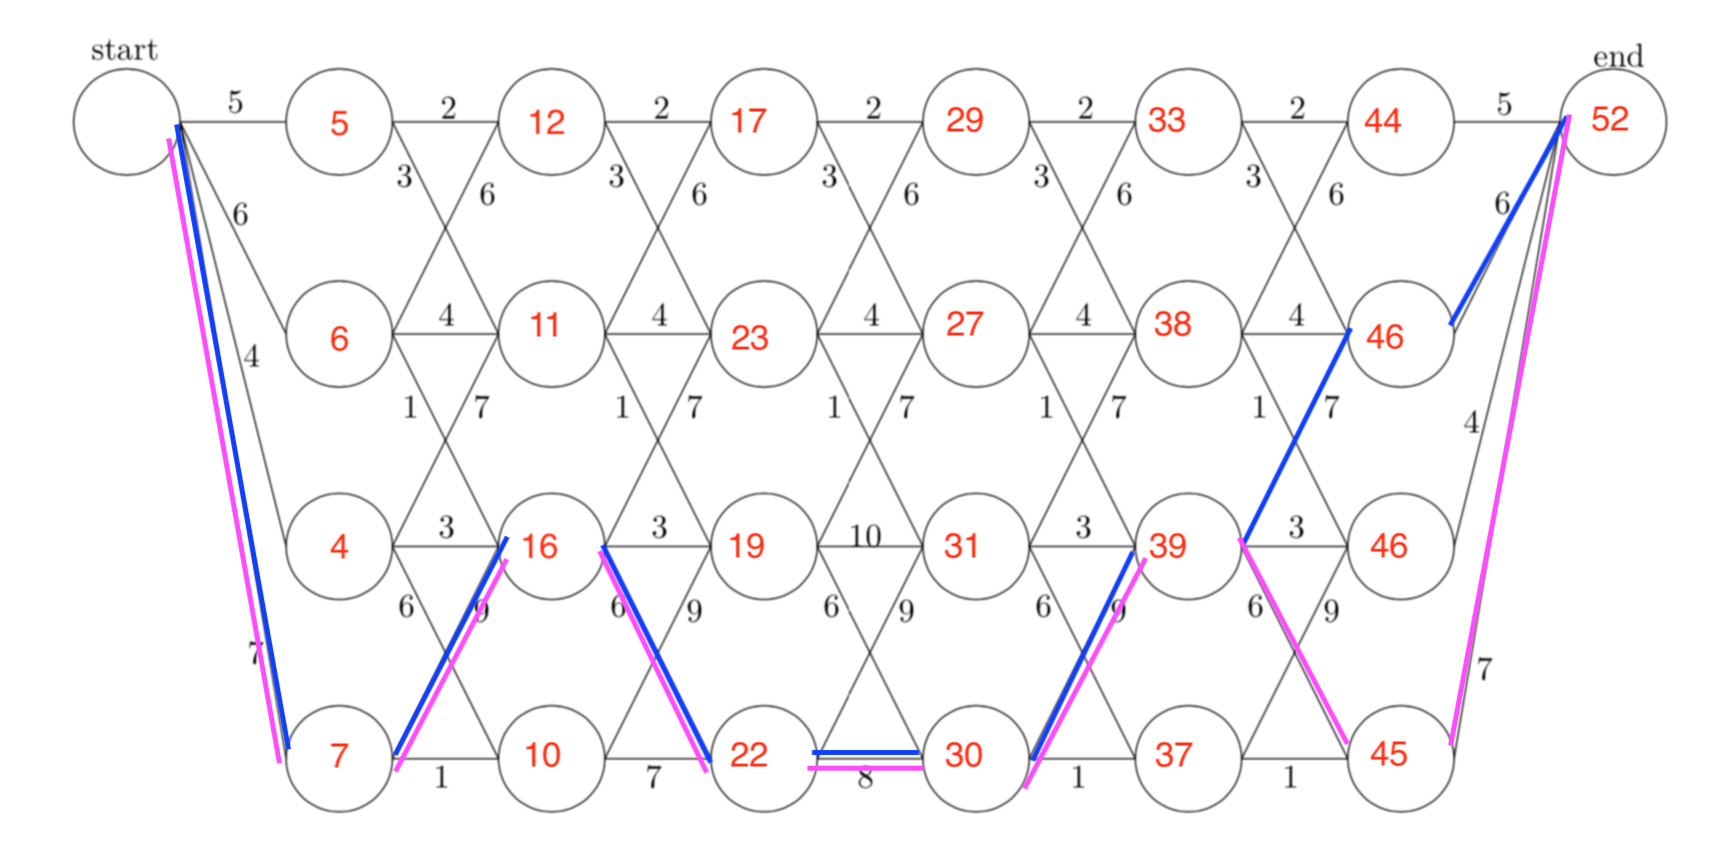
\includegraphics[width=1.0\textwidth]{prob1_2}
\caption{Longest Path}
\end{figure}





%%%%%%%%%%%%%%%%%%%%%%
\section*{Problem 2}


\subsection*{(a)}
By Bellman's Expectation equation:
\begin{align*}
V_{\pi}(s) &= \sum_a \pi(a | s) q_{\pi}(s,a); \\
q_{\pi}(s,a) & = R_s^a + \gamma \sum_{s^{'}} P_{s s^{'}}^{(a)} V_{\pi}(s^{'}).
\end{align*}
Therefore:
\begin{align*}
V_{\pi}(0) & = q_{\pi}(0,1) = R_0^1 + \gamma (P_{00}^{(1)} V_{\pi}(0) + P_{01}^{(1)} V_{\pi}(1) ); \\
V_{\pi}(1) & = q_{\pi}(1,2) = R_1^2 + \gamma (P_{10}^{(2)} V_{\pi}(0) + P_{11}^{(2)} V_{\pi}(1) ).
\end{align*}
Thus $(V_{\pi}(0), V_{\pi}(1)) = (5.6, 6.4)$.


\subsection*{(b)}
\begin{align*}
V_{\pi}^{(t+1)}(0) & \leftarrow R_0^1 + \gamma (P_{00}^{(1)} V_{\pi}^{(t)}(0) + P_{01}^{(1)} V_{\pi}^{(t)}(1) ); \\
V_{\pi}^{(t+1)}(1) & \leftarrow R_1^2 + \gamma (P_{10}^{(2)} V_{\pi}^{(t)}(0) + P_{11}^{(2)} V_{\pi}^{(t)}(1) ).
\end{align*}
Let  $(V_{\pi}^{(0)}(0), V_{\pi}^{(0)}(1)) = (0, 0)$, then:

\begin{align*}
 (V_{\pi}^{(1)}(0), V_{\pi}^{(1)}(1)) &= (2.25, 3); \\
 (V_{\pi}^{(2)}(0), V_{\pi}^{(2)}(1)) &= (3.0625, 3.875); \\
 (V_{\pi}^{(3)}(0), V_{\pi}^{(3)}(1)) &= (3.703125, 4.5); \\
 (V_{\pi}^{(4)}(0), V_{\pi}^{(4)}(1)) &= (4.175781, 4.976562); \\
 (V_{\pi}^{(5)}(0), V_{\pi}^{(5)}(1)) &= (4.532227, 5.332031); \\
 (V_{\pi}^{(100)}(0), V_{\pi}^{(100)}(1)) &= (5.6, 6.4).
\end{align*}

\subsection*{(c)}
\begin{equation}
\left(                     
\begin{matrix}
q_{\pi}(0,1) \\  q_{\pi}(1,1) \\  q_{\pi}(0,2) \\  q_{\pi}(1,2)
\end{matrix}
\right) =
\left(                     
\begin{matrix}
R_0^1 \\ R_q^1 \\ R_0^2 \\ R_1^2 
\end{matrix}
\right)  + \gamma
\left(                     
\begin{matrix}
P_{00}^{(1)} & 0 & 0 & P_{01}^{(1)} \\
P_{10}^{(1)} & 0 & 0 & P_{11}^{(1)} \\
P_{00}^{(2)} & 0 & 0 & P_{01}^{(2)} \\
P_{10}^{(2)} & 0 & 0 & P_{11}^{(2)} 
\end{matrix}
\right) 
\left(                     
\begin{matrix}
R_0^1 \\ R_q^1 \\ R_0^2 \\ R_1^2 
\end{matrix}
\right) 
\end{equation}
Then $(q_{\pi}(0,1),  q_{\pi}(1,1),  q_{\pi}(0,2),  q_{\pi}(1,2) ) = (5.6, 7.65, 8.5, 6.4)$.


\subsection*{(d)}

$$\because \ \pi^{'}(s) = \mathrm{arg} \max_{a} q_{\pi}(s, a)$$
$$\therefore \ \pi^{'}(0) = 2; \ \pi^{'}(1) = 1. $$

\subsection*{(e)}

By Bellman?s optimality equation: $$V_{*}(s) = \max_{a} \bigg(R_s^a + \gamma \sum_{s^{'}}  P_{s s^{'}}^{(a)} V_{*}(s^{'}) \bigg),$$
therefore let:
\begin{align*}
V_{*}^{(t+1)}(0) &\leftarrow \max_a \bigg(  R_0^a + \gamma P_{00}^{(a)} V_{*}^{(t)}(0) +   \gamma P_{01}^{(a)} V_{*}^{(t)}(1)  \bigg) ; \\
V_{*}^{(t+1)}(1) &\leftarrow \max_a \bigg(  R_1^a + \gamma P_{10}^{(a)} V_{*}^{(t)}(0) +   \gamma P_{11}^{(a)} V_{*}^{(t)}(1)  \bigg).
\end{align*}
therefore:
$$ (V_{*}^{(100)}(0), V_{*}^{(100)}(1)) = (14.154,  12.923). $$


\subsection*{(f)}
\begin{align*}
\pi_{*}(0) = \mathrm{arg} \max_a \bigg(  R_0^a + \gamma P_{00}^{(a)} V_{*}^{(t)}(0) +   \gamma P_{01}^{(a)} V_{*}^{(t)}(1)  \bigg) =  2; \\
\pi_{*}(1) = \mathrm{arg} \max_a \bigg(  R_1^a + \gamma P_{10}^{(a)} V_{*}^{(t)}(0) +   \gamma P_{11}^{(a)} V_{*}^{(t)}(1)  \bigg) =  1. \\
\end{align*}




%%%%%%%%%%%%%%%%%%%%%%
\section*{Problem 3}

\subsection*{(a), (b), (c)}

The estimated value function $v_{\pi}(s)$ based on Monte Carlo policy evaluation method is: 
$$  (v_{\pi}(0), v_{\pi}(1)) = (5.59, 6.40). $$
The estimated value function $v_{\pi}(s)$ based on  5-step temporal difference policy evaluation method is:
$$  (v_{\pi}(0), v_{\pi}(1)) = (5.59, 6.39). $$

\subsection*{(d), (e)}
The optimal action-value function $q_{*}(s, a)$ estimated based on SARSA algorithm is:
$$ (q_{*}(0, 1), q_{*}(0, 2), q_{*}(1, 1), q_{*}(1, 2)) = (9.27, 13.12, 11.88, 10.93). $$
The optimal action-value function $q_{*}(s, a)$ estimated based on Q-learning algorithm is:
$$ (q_{*}(0, 1), q_{*}(0, 2), q_{*}(1, 1), q_{*}(1, 2)) = (8.49, 13.50, 12.28, 10.35). $$
Both of the methods indicate that:

\begin{equation*}
\left\{
\begin{aligned}
\pi_{*}(0) &=  2; \\
\pi_{*}(1) &=  1. 
\end{aligned}
\right.
\end{equation*}



\end{document}













